\documentclass[a4paper,10pt]{article}
\usepackage[utf8]{inputenc}
\usepackage{graphicx}
\usepackage{subcaption}

\usepackage{graphicx}
\usepackage{hyperref}

\usepackage{pstricks}
\usepackage{pst-node}
\usepackage{wrapfig}

\usepackage{listings}
\lstset{language=C,basicstyle=\scriptsize\color{green},identifierstyle=\color{orange},keywordstyle=\color{blue}}

\usepackage{amsmath}
\usepackage{amssymb}
\bibliographystyle{plain}

\begin{document}
%%%%%%%%%%%%%%%%%%%%%%%%%%%%%%%%%%%%%%%%%%%%%%%%%%%%%%%%%%%%%%%%%%%%%%%%%%%%%%%%%%%%%%%%%
%=======================================================================================%
%%%%%%%%%%%%%%%%%%%%%%%%%%%%%%%%%%%%%%%%%%%%%%%%%%%%%%%%%%%%%%%%%%%%%%%%%%%%%%%%%%%%%%%%%
\begin{titlepage}
%%%%%%%%%%%%%%%%%%%%%%%%%%  LOGO  %%%%%%%%%%%%%%%%%%%%%%%%%%%%%%%%%%%%%%%%%
 \begin{pspicture}(-5,4)(5,5)
%\rput(-5,3){\href{http://www.upmc.fr/FR/info/00}{
\includegraphics[scale=1.0]{upmc_logo}}}
\rput(-4,6.5){
\includegraphics[scale=1.0]{upmc_logo}}
\rput(-4,5){\resizebox{6cm}{0.3cm}{\begin{tabular}{l}
		Université de Pierre et Marie CURIE (PARIS VI) \\
		4 Place Jussieu 75005 Paris
            \end{tabular}}}
%\psline(-5,0)(5,0)
\end{pspicture}
%%%%%%%%%%%%%%%%%%%%%%%%%%  LOGO  %%%%%%%%%%%%%%%%%%%%%%%%%%%%%%%%%%%%%%%%%
%%%%%%%%%%%%%%%%%%%%%%%%%%  Titre %%%%%%%%%%%%%%%%%%%%%%%%%%%%%%%%%%%%%%%%%
\begin{center}
\resizebox{14cm}{1cm}{Laminar flow in a pipe}\\ 
\large{Stationar Navier-Stokes's equation}\\
\large\textbf{Directed by M.Fr\'{e}d\'{e}ric Hecht}
\end{center}
%%%%%%%%%%%%%%%%%%%%%%%%%%  Titre  %%%%%%%%%%%%%%%%%%%%%%%%%%%%%%%%%%%%%%%%%
%%%%%%%%%%%%%%%%%%%%%%%%%%  image maillage %%%%%%%%%%%%%%%%%%%%%%%%%%%%%%%%
\begin{pspicture}(-7,-2)(7,2)
\psline[linecolor=blue](5,1)(-5,1)%Label = 2
\rput(0,1.25){\Rnode{C}{\small{\color{blue}label=2}}}
\psline[linecolor=red](-5,1)(-5,0)%Label = 1
\rput(-5,1.25){\small $\beta$} \rput(-5,-0.25){\small $\alpha$}
\rput{90}(-5.25,0.5){\Rnode{D}{\small{\color{red}label=1}}}
\psline[linecolor=blue](-5,0)(-3,0)(-3,-1)(5,-1)%Label = 2
\rput(0,-1.25){\Rnode{E}{\small{\color{blue}label=2}}}
\pscurve[linecolor=green](5,-1)(4.75,-0.5)(5.1,0)(4.5,0.5)(5,1)%Label = 3
\rput{-90}(5.5,0){\Rnode{F}{\small{\color{green}label=3}}}


\pscurve[linecolor=red](-5,0)(-4,0.5)(-5,1)%Label = 3
\rput(-4.75,0.75){\Rnode{A}{}}
\rput(-6,1.9){\Rnode{B}{\color{red}\small 4*(y-$\alpha$)*($\beta$-y)}}
\ncline{->}{A}{B}
%\psline(-7,-2)(7,2)
\end{pspicture}
%%%%%%%%%%%%%%%%%%%%%%%%%%  image maillage %%%%%%%%%%%%%%%%%%%%%%%%%%%%%%%%%%%%
%%%%%%%%%%%%%%%%%%%%%%%%%%  Auteur %%%%%%%%%%%%%%%%%%%%%%%%%%%%%%%%%%%%%%%%%
\begin{flushright}
\underline{\textbf {NGUYEN Chi Thanh}} \\
{\textbf {2008-2009}}
\end{flushright}
%%%%%%%%%%%%%%%%%%%%%%%%%%  Auteur %%%%%%%%%%%%%%%%%%%%%%%%%%%%%%%%%%%%%%%%%
\begin{center}
\begin{pspicture}(-7,-4)(7,4)
\rput(-3,-5){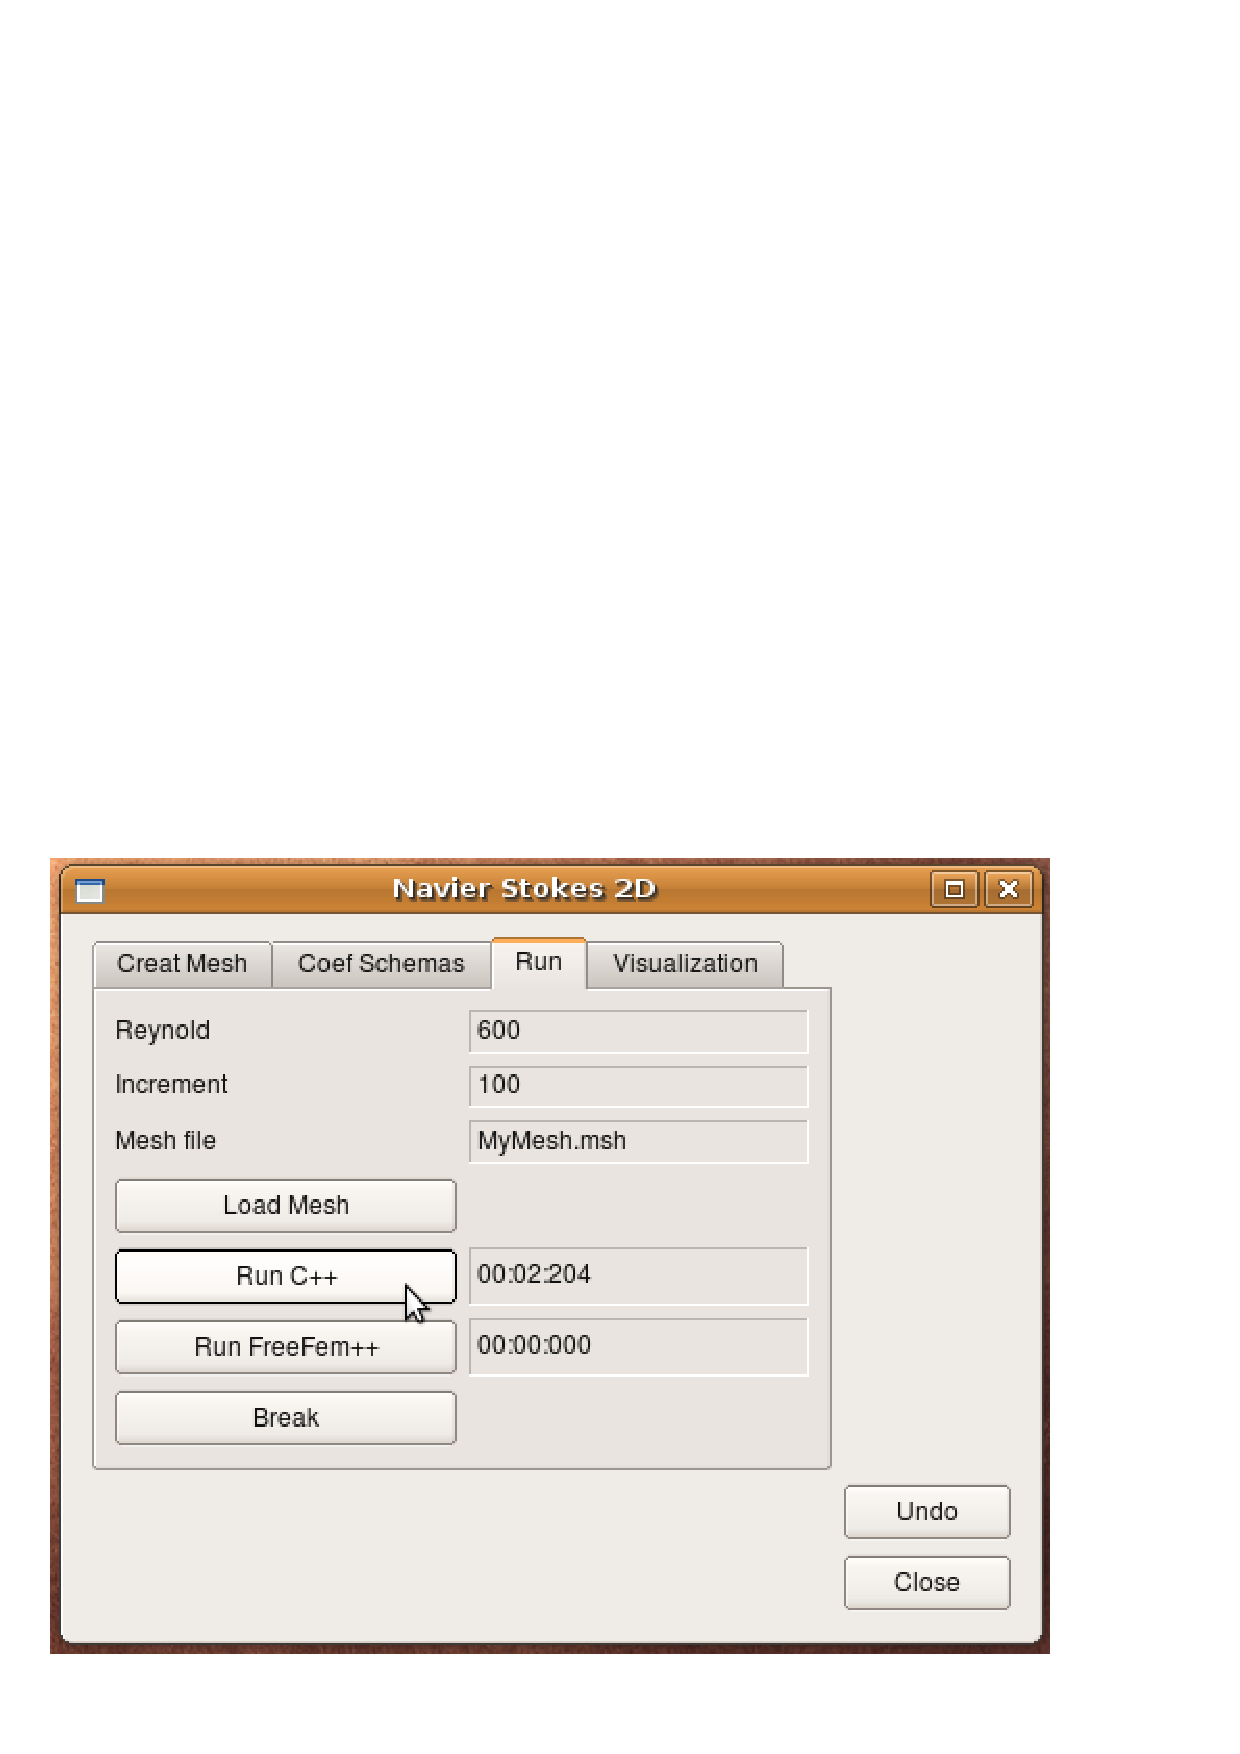
\includegraphics[scale=0.5]{ImageTitle}}
\rput(4.7,3){\begin{tabular}{l}
		$\bullet$  \texttt{existence and uniqueness} \\
		$\bullet$  \texttt{Continuation method} \\
		$\bullet$  \texttt{C++ Programming} \\
		$\bullet$  \texttt{Qt GUI Programming} 	
               \end{tabular}}
%\psline(-7,-4)(7,7)
\end{pspicture}
\end{center}

\end{titlepage}
\tableofcontents
%%%%%%%%%%%%%%%%%%%%%%%%%%%%%%%%%%%%%%%%%%%%%%%%%%%%%%%%%%%%%%%%%%%%%%%%%%%%%%%%%%%%%%%%%
%=======================================================================================%
%%%%%%%%%%%%%%%%%%%%%%%%%%%%%%%%%%%%%%%%%%%%%%%%%%%%%%%%%%%%%%%%%%%%%%%%%%%%%%%%%%%%%%%%%
\section*{Introduction}
In the studies of Master 2 mathematical modeling (ANEDP) at the Pierre and Marie Curie University, students following the NM406 module (PDE's resolution by the Finite Element Method) taught by\href{http://www.ann.jussieu.fr/~hecht/}{M. Fr\'{e}d\'{e}ric Hecht} must complete a scienfic computing project using the FEM developed in C ++. This project is based on the library used to develop the software \href {http://www.freefem.org/ff++/}{FreeFem++} by the teacher.

\paragraph{Physical phenomenon : } The project is to simulate laminar flow in a pipe by solving the stationary Navier-Stokes equation. Laminar flow is regular (it does not have too much spatial or temporal variations), often stationary. The viscosity stabilizes and regulates generally flows. A fluid having a high viscosity will flow in a laminar manner. A flow is characterized by the Reynolds number, which allows you to get an idea of stability: When this number is low, the flow is laminar when it is high, the flow is unstable and turbulent general. The transition between stable and unstable or turbulent flow is an important study subject. In a pipe, it is often assumed that the transition can occur between 2000 and 3000.

\paragraph{Mathematical problem :} This is in fact a stable solution of the Navier-Stokes equations, in the sense that if one modifies the flow, returns to the laminar solution. The area studied here is a classic problem: the downward stair.
\begin{center}
 \begin{pspicture}(-7,-1.5)(7,1.5)
 \psline[linecolor=blue](5,1)(-5,1)
 \psline[linecolor=red](-5,1)(-5,0)
 \rput(-5.25,0.5){\color{red}$\Gamma$}
 \psline[linecolor=blue](-5,0)(-3,0)(-3,-1)(5,-1)
 \pscurve[linecolor=green](5,-1)(4.75,-0.5)(5.1,0)(4.5,0.5)(5,1)
 \pscurve[linecolor=red](-5,0)(-4,0.5)(-5,1)
 %\psline(-7,-1.5)(7,1.5)
 \end{pspicture}
\end{center}
The entrance of the fluid from the right with the parabolic Poiseuille profit represent the Poiseuille's condition, giving the following mathematical problem :
\[
(\wp)\hspace{0.25cm}\left\{
\begin{array}{rl}
(\textbf{u}.\triangledown) \textbf{u} -\nu \bigtriangleup \textbf{u} + \triangledown p & =0 \\
\triangledown \textbf{u} & =0 \\
\textbf{u}_\Gamma &=g 
\end{array}\right.
\]
Mainly aims to solve this problem, the project is therefore composed of the mathematical study (existence and uniqueness of solution, numerical implementation), and computer-based learning C ++ programming to solve this problem.
\section{Mathematical study}
%\bibliography{ReferenceNCT}
%\nocite{*}
\end{document}



